\documentclass[12pt]{article}
\usepackage{amsmath,amssymb,siunitx}
\usepackage{tikz}
\usepackage{circuitikz}

\usepackage[margin=1in]{geometry}
\begin{document}

\begin{enumerate}

\item A uniformly charged ring of radius $R$ carries total charge $Q$. The axial field at distance $x$ is $E(x)=\dfrac{1}{4\pi\varepsilon_0}\dfrac{Qx}{(x^2+R^2)^{3/2}}$. By differentiating and carefully analysing the extremum including sign of second derivative, determine both the position and the corresponding maximum field magnitude.\\

% Diagram for Question 1
\begin{center}
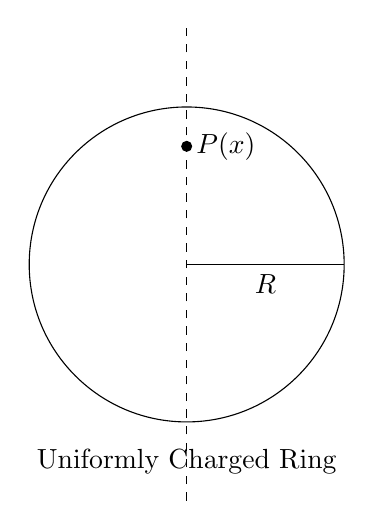
\begin{tikzpicture}[scale=1]

% Ring
\draw (0,0) circle (2);

% Axis
\draw[dashed] (0,-3) -- (0,3);

% Point on axis
\fill (0,1.5) circle (2pt);
\node[right] at (0,1.5) {$P(x)$};

% Radius marking
\draw (0,0) -- (2,0);
\node[below] at (1,0) {$R$};

\node at (0,-2.5) {Uniformly Charged Ring};

\end{tikzpicture}
\end{center}


A) $x=\dfrac{R}{\sqrt{2}},\; E_{\max}=\dfrac{1}{4\pi\varepsilon_0}\dfrac{2Q}{3\sqrt{3}R^2}$\\

B) $x=R,\; E_{\max}=\dfrac{1}{4\pi\varepsilon_0}\dfrac{Q}{2R^2}$\\

C) $x=\dfrac{R}{\sqrt{3}},\; E_{\max}=\dfrac{1}{4\pi\varepsilon_0}\dfrac{Q}{3R^2}$\\

D) $x=\dfrac{R}{\sqrt{2}},\; E_{\max}=\dfrac{1}{4\pi\varepsilon_0}\dfrac{Q}{3\sqrt{3}R^2}$


\item A parallel plate capacitor of capacitance $C_0$ is connected to a battery of emf $V$. A dielectric slab of dielectric constant $K$ is inserted slowly, but the battery has internal resistance $r$ and insertion takes time $t$ comparable to $RC_0$. Considering charge flow through resistance and final steady state, determine the net heat dissipated in the resistor during insertion.\\

% Diagram for Question 2
\begin{center}
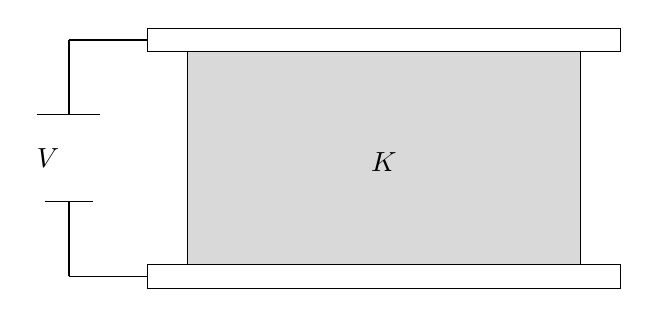
\begin{tikzpicture}[scale=1]

% Plates
\draw (-3,0) rectangle (3,0.3);
\draw (-3,3) rectangle (3,3.3);

% Dielectric slab
\draw[fill=gray!30] (-2.5,0.3) rectangle (2.5,3);

\node at (0,1.6) {$K$};

% Wires to battery
\draw (-3,0.15) -- (-4,0.15);
\draw (-3,3.15) -- (-4,3.15);

% Battery symbol
\draw (-4,0.15) -- (-4,1.1);
\draw (-4,2.2) -- (-4,3.15);

% Battery plates
\draw (-4.3,1.1) -- (-3.7,1.1);   % short plate
\draw (-4.4,2.2) -- (-3.6,2.2);   % long plate

\node[left] at (-4,1.65) {$V$};



\end{tikzpicture}
\end{center}

A) $\dfrac{1}{2}C_0V^2(K-1)$\\

B) $\dfrac{1}{2}C_0V^2(K-1)^2$\\

C) $\dfrac{1}{2}C_0V^2(K^2-1)$\\

D) Zero

\item A rectangular loop of width $l$ and resistance $R$ enters a uniform magnetic field $B$ region with constant velocity $v$. During entry, induced current produces magnetic force opposing motion; external agent maintains constant speed. By integrating power supplied by external agent over time of entry, determine total work done and hence total charge passed through loop.\\

% Diagram for Question 3
\begin{center}
\begin{tikzpicture}[scale=1]

% Loop
\draw (0,0) rectangle (2,2);

% Velocity arrow
\draw[->,thick] (2.3,1) -- (4,1);
\node[above] at (3.2,1) {$v$};

% Magnetic field region
\draw (4,0) rectangle (7,2);
\node at (5.5,2.6) {$B$};

% Cross marks for B into page
\foreach \x in {4.5,5.5,6.5}
  \foreach \y in {0.5,1.5}
    \node at (\x,\y) {$\times$};

\end{tikzpicture}
\end{center}

A) $Q=\dfrac{Bl^2}{R}$\\

B) $Q=\dfrac{Blv}{R}$\\

C) $Q=\dfrac{Bl^2v}{R}$\\

D) $Q=0$

\item A long solenoid of inductance $L_0$ carries constant current $I$. An iron core of relative permeability $\mu_r$ is inserted fully while current is maintained constant by ideal source. Considering change in magnetic field, energy density, and work done by source, determine increase in magnetic energy stored.\\

A) $\dfrac{1}{2}L_0I^2(\mu_r-1)$\\

B) $\dfrac{1}{2}L_0I^2(\mu_r^2-1)$\\

C) $\dfrac{1}{2}L_0I^2\left(1-\dfrac{1}{\mu_r}\right)$\\

D) Zero


\item In an RC circuit connected to constant voltage $V$, capacitor voltage grows as $V(1-e^{-t/RC})$. Determine time at which rate of increase of electrostatic energy stored in capacitor becomes maximum, and evaluate that time in terms of $RC$.\\

A) $RC\ln 2$\\

B) $RC$\\

C) $RC\ln\sqrt{2}$\\

D) $RC/2$


\item An AC bridge has arms $Z_1=R$, $Z_2=\dfrac{1}{j\omega C}$, $Z_3=R$, $Z_4=j\omega L$. Using complex impedance balance condition and separating real and imaginary parts, determine frequency at which bridge balances.\\

% Diagram for Question 6
\begin{center}

\begin{circuitikz}

% Left vertical
\draw (0,0) to[R=$R$] (0,3);

% Top horizontal
\draw (0,3) to[C=$C$] (3,3);

% Right vertical
\draw (3,3) to[R=$R$] (3,0);

% Bottom horizontal
\draw (3,0) to[L=$L$] (0,0);

% Bridge diagonal (detector branch placeholder)
\draw[dashed] (0,3) -- (3,0);

\end{circuitikz}


\end{center}

A) $\omega=\dfrac{1}{\sqrt{LC}}$\\

B) $\omega=\dfrac{R}{L}$\\

C) $\omega=\dfrac{1}{RC}$\\

D) $\omega=\dfrac{R}{\sqrt{LC}}$


\item An electron enters perpendicular electric and magnetic fields such that net force is zero and it moves straight. If magnetic field increases slowly while electric field remains fixed, determine nature of trajectory immediately after imbalance and radius of curvature in terms of $E,B,m,e$.\\

% Diagram for Question 7
\begin{center}
\begin{tikzpicture}[scale=1]

% Velocity
\draw[->,thick] (0,0) -- (3,0);
\node[below] at (1.5,0) {$v$};

% Electric field
\draw[->,thick] (0,0) -- (0,2);
\node[left] at (0,1) {$E$};

% Magnetic field into page
\node at (2,1) {$\times$};
\node at (2.5,1.5) {$\times$};
\node at (1.5,1.5) {$\times$};

\node[right] at (2.8,1.8) {$B$};

\end{tikzpicture}
\end{center}

A) Circular of radius $\dfrac{mE}{eB^2}$\\

B) Straight line\\

C) Helical of radius $\dfrac{mE}{eB^2}$\\

D) Parabolic


\item In an ideal LC circuit, charge varies as $Q=Q_0\cos\omega t$. Since electric energy varies as $Q^2$ and magnetic energy as $I^2$, determine angular frequency of oscillation of electric energy and hence time interval between two successive maxima of electric energy.\\

A) $2\omega,\; \dfrac{\pi}{\omega}$\\

B) $\omega,\; \dfrac{2\pi}{\omega}$\\

C) $2\omega,\; \dfrac{\pi}{2\omega}$\\

D) $\omega,\; \dfrac{\pi}{\omega}$


\item A transformer with primary turns $N_p$ and secondary turns $N_s$ supplies power to load $R_L$. If secondary turns are doubled while primary remains same and input voltage fixed, determine percentage change in current drawn from primary assuming ideal transformer.\\

% Diagram for Question 9
\begin{center}
\begin{tikzpicture}[scale=1]

% Transformer core
\draw (-1,0) -- (-1,3);
\draw (4,0) -- (4,3);

% Primary coil
\draw (-2,0.5) to[american inductor] (-2,2.5);
\node[left] at (-2,1.5) {$N_p$};

% Secondary coil
\draw (5,0.5) to[american inductor] (5,2.5);
\node[right] at (5,1.5) {$N_s$};

\draw (-2,0.5) -- (-1,0.5);
\draw (-2,2.5) -- (-1,2.5);

\draw (5,0.5) -- (4,0.5);
\draw (5,2.5) -- (4,2.5);

\end{tikzpicture}
\end{center}

A) 100\% increase\\

B) 50\% decrease\\

C) 100\% decrease\\

D) No change


\item In photoelectric effect experiment, stopping potential versus frequency graph has slope $h/e$. If stopping potential increases by $1\,\text{V}$ when frequency increases by $2.4\times10^{14}\,\text{Hz}$, determine Planck’s constant. $(e=1.6\times10^{-19}\,\text{C})$\\

% Diagram for Question 10
\begin{center}
\begin{tikzpicture}[scale=1]

% Axes
\draw[->] (0,0) -- (5,0) node[right] {$\nu$};
\draw[->] (0,0) -- (0,3.5) node[above] {$V_0$};

% Line
\draw[thick] (1,0) -- (4.5,2.8);

% Threshold frequency
\draw[dashed] (1,0) -- (1,-0.2);
\node[below] at (1,-0.2) {$\nu_0$};

\node at (3.5,3.0) {Slope $=\dfrac{h}{e}$};

\end{tikzpicture}
\end{center}

A) $6.4\times10^{-34}\,\text{J·s}$\\

B) $3.8\times10^{-34}\,\text{J·s}$\\

C) $6.6\times10^{-34}\,\text{J·s}$\\

D) $1.6\times10^{-19}\,\text{J·s}$

\item When dielectric is inserted in capacitor connected to constant voltage source, stored energy increases but electric field inside decreases. The additional energy supplied by battery equals\\

A) Increase in stored energy plus heat dissipated\\

B) Increase in stored energy only\\

C) Decrease in stored energy\\

D) Zero

\item A magnetic dipole in non-uniform magnetic field experiences both torque and force. In uniform magnetic field, translational force is zero because force depends on\\

A) Gradient of magnetic field\\

B) Magnitude only\\

C) Flux\\

D) Dipole length

\item A conducting loop moves entirely within uniform magnetic field without changing its orientation or area. Even though charges experience magnetic force, no net emf is induced because\\

A) Net magnetic flux remains constant\\

B) Magnetic force zero\\

C) Resistance infinite\\

D) Electric field absent

\item In purely resistive AC circuit, instantaneous power averaged over one cycle equals $V_{rms}I_{rms}$. This occurs because phase difference between voltage and current is\\

A) Zero\\

B) $\pi/2$\\

C) $\pi$\\

D) Variable

\item Hall voltage in a conductor of thickness $t$, current $I$, magnetic field $B$, and carrier density $n$ is $V_H=\dfrac{BI}{net}$. If both current and magnetic field are doubled while thickness is halved, determine factor by which Hall voltage changes.\\

A) 8\\

B) 4\\

C) 2\\

D) 16

\end{enumerate}

\end{document}